% Created 2018-09-29 Sat 11:29
\documentclass[9pt, b5paper]{article}
\usepackage{fontspec}
\usepackage{graphicx}
\usepackage{xcolor}
\usepackage[slantfont,boldfont]{xeCJK}
\setCJKmainfont[BoldFont = Heiti SC, ItalicFont = STFangsong]{STSong}
\setCJKsansfont{STHeiti}
\setCJKmonofont{STFangsong}
\usepackage{multirow}
\usepackage{multicol}
\usepackage{float}
\usepackage{textcomp}
\usepackage{geometry}
\geometry{left=0.1cm,right=0.1cm,top=0.1cm,bottom=0.1cm}
\usepackage{algorithm}
\usepackage{algorithmic}
\usepackage{latexsym}
\usepackage{natbib}
\usepackage{listings}
\usepackage{minted}
\usepackage[xetex,colorlinks=true,CJKbookmarks=true,linkcolor=blue,urlcolor=blue,menucolor=blue]{hyperref}
\author{deepwaterooo}
\date{\today}
\title{Unity shader 渲染进界:细节或框架理解升华}
\hypersetup{
  pdfkeywords={},
  pdfsubject={},
  pdfcreator={Emacs 25.3.1 (Org mode 8.2.7c)}}
\begin{document}

\maketitle
\tableofcontents


\section{Unity Shader入门精要笔记(一):渲染流水线}
\label{sec-1}
\begin{itemize}
\item \url{https://blog.csdn.net/lzhq1982/article/details/73312811}
\end{itemize}
\subsection{一个渲染流程分为3个阶段}
\label{sec-1-1}
\begin{itemize}
\item 应用阶段(Application Stage): cpu负责,由开发者准备好摄像机,模型,光源等数据,做好粗粒度的剔除工作,并设置好材质,纹理,shader等渲染状态,最后输出渲染所需要的图元的过程。
\item 几何阶段(Geometry Stage): gpu负责,把上个阶段传过来的图元进行逐顶点,逐多边形的操作。把顶点坐标从模型空间经过一系列转换最终到屏幕空间,输出屏幕空间二维顶点坐标,顶点深度、着色等数据,交给光栅器处理。
\item 光栅化阶段(Rasterizer Stage): gpu负责,对上个阶段的逐顶点数据(纹理坐标、顶点颜色等)进行插值,再逐像素处理,决定哪些像素应该被绘制在屏幕上,并计算他们的颜色。
\end{itemize}
\subsection{CPU和GPU的通信}
\label{sec-1-2}
\subsubsection{cpu的工作:把数据加载到显存,设置渲染状态,调用draw call。}
\label{sec-1-2-1}
\begin{itemize}
\item 把数据加载到缓存:所有数据都要从硬盘加载到系统内存,然后网格和纹理,顶点位置、颜色,法线,纹理坐标等数据加载到显存中。
\item 设置渲染状态:使用哪个顶点着色器和片元着色器,光源属性,材质等来渲染的过程,渲染状态不改,所有网格都会使用一种渲染状态。
\item 调用draw call:翻译过来就是绘制命令,由cpu发出,指向一个要被渲染的图元列表,通知gpu可以按照上面的设置渲染这些图元了。我们常说优化draw call,是因为cpu准备上述数据是个复杂的过程,而gpu绘制却很快,如果draw call很频繁,cpu光顾着准备数据了,gpu又空等着,结果可想而知,所以每次发出draw call,我们应该尽可能多准备数据给gpu,这样就可以用尽量少的draw call达到通知gpu快速渲染的效果。可是如何调一次draw call尽可能多准备数据给gpu呢,这需要一个专门的主题了。
\end{itemize}
\subsubsection{GPU流水线}
\label{sec-1-2-2}
\begin{figure}[htb]
\centering
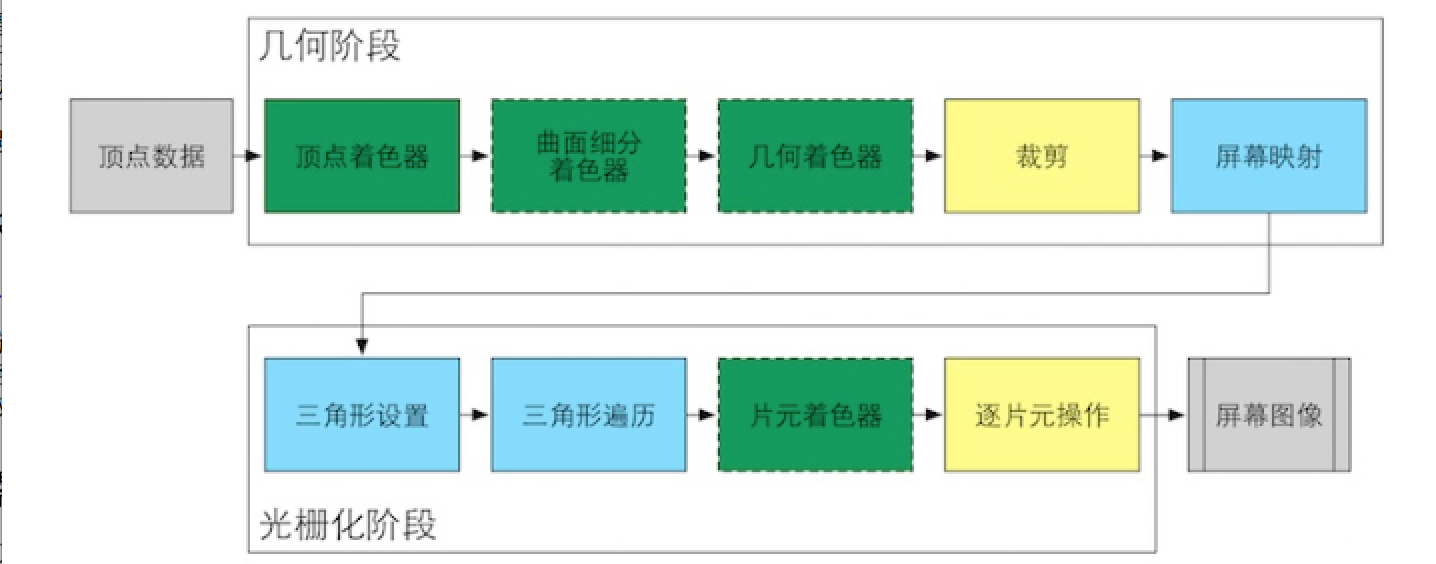
\includegraphics[width=.9\linewidth]{./pic/gpuPipeline.png}
\caption{GPU流水线}
\end{figure}
\begin{itemize}
\item 上图中绿色表示该流水线是完全可编程控制的,黄色表示可以配置但不可以编程的,蓝色表示GPU固定实现的,开发者没有控制权。虚线框表示该shader是可选的。
\item 下面我们逐一看一下:
\end{itemize}
\begin{enumerate}
\item 顶点着色器
\label{sec-1-2-2-1}
\begin{itemize}
\item 顶点着色器:写shader人员必须要面对的重点部分。顾名思义,该阶段处理的是顶点数据,重点是这里是单个顶点数据,你别想访问其他顶点数据。我们要在这里完成顶点的坐标变换,把顶点从模型空间转换到齐次裁剪空间,再经透视除法,最终得到归一化设备坐标(NDC)。还有逐顶点光照,并准备好后面阶段需要的其他数据,比如纹理坐标,顶点颜色等。

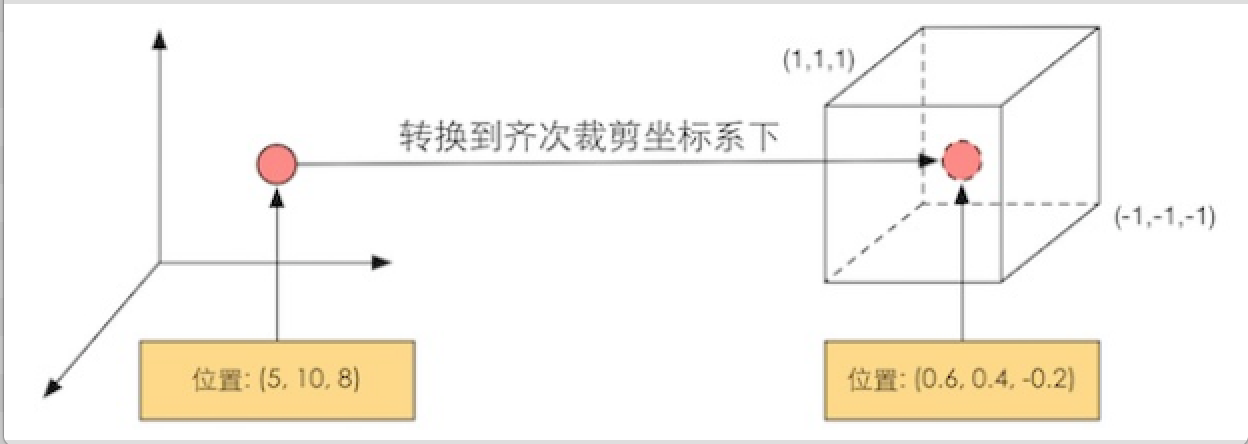
\includegraphics[width=.9\linewidth]{./pic/vertex.png}
\end{itemize}
\item 曲面细分着色器
\label{sec-1-2-2-2}
\begin{itemize}
\item 曲面细分着色器: 用于细分图元,几何着色器用于执行逐图元的着色操作,或产生更多图元,这两个阶段都是可选的。
\end{itemize}
\item 裁剪
\label{sec-1-2-2-3}
\begin{itemize}
\item 裁剪:上面阶段我们得到的NDC是立方体空间,Unity,OpenGL是从(-1,-1,-1)到(1,1,1),DirectX的z是从0到1,完全在该空间内的图元保留,完全在外面的抛弃,一半在内一半在外的就需要裁剪了,这就是我们视野内的部分。该阶段是可配置的,比如我们用自定义的裁剪平面,或裁剪图元的正面或背面。

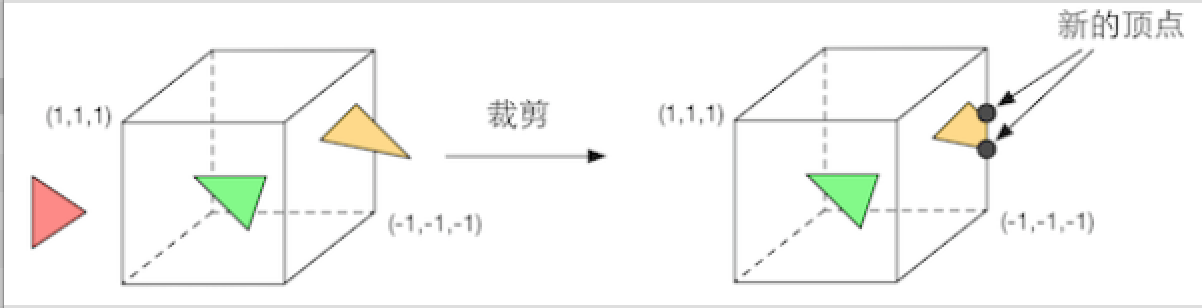
\includegraphics[width=.9\linewidth]{./pic/clip.png}
\end{itemize}
\item 屏幕映射
\label{sec-1-2-2-4}
\begin{itemize}
\item 屏幕映射:该阶段是不可配置和编程的。这里输入的坐标是三维的,屏幕映射的任务是把每个图元的x,y坐标转换到屏幕坐标系(二维)下,前面NDC我们的x,y在(-1,1)内,所以映射到屏幕上就是个缩放的过程,而最终的屏幕坐标系会和z坐标构成窗口坐标系,传给光栅化阶段。有一点要注意,OpenGL会以屏幕左下角为最小坐标,而DirectX会以左上角为最小坐标。

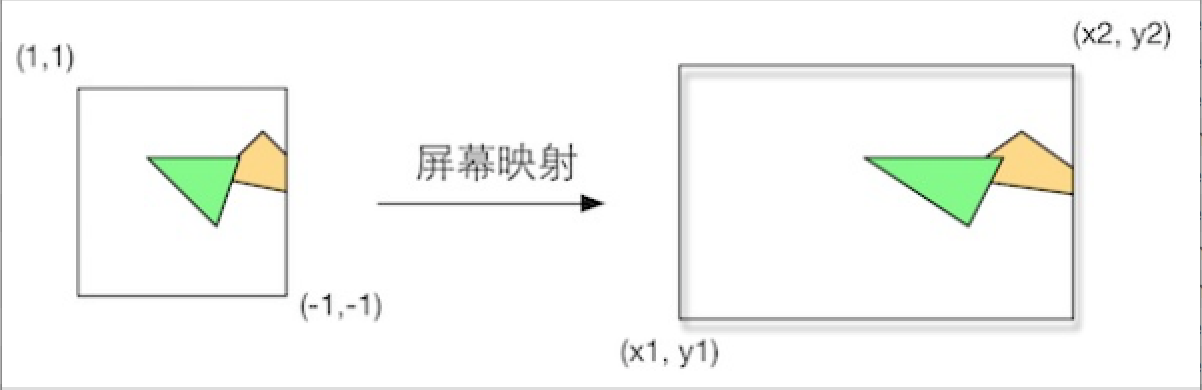
\includegraphics[width=.9\linewidth]{./pic/reflection.png}
\end{itemize}
\item 三角形设置
\label{sec-1-2-2-5}
\begin{itemize}
\item 三角形设置:不可配置和编程。从这一步开始进入光栅化阶段。上个阶段输出的都是三角形顶点,而这个阶段我们要用这些顶点和计算出来的三角形边界组成三角形网格数据。
\end{itemize}
\item 三角形遍历
\label{sec-1-2-2-6}
\begin{itemize}
\item 三角形遍历:不可配置和编程。检查每个像素被哪个三角形所覆盖,而后生成片元,重点是三角形的三个顶点会对覆盖的每个像素的数据进行插值,比如深度和坐标等,记住这点很重要,如下图所示:

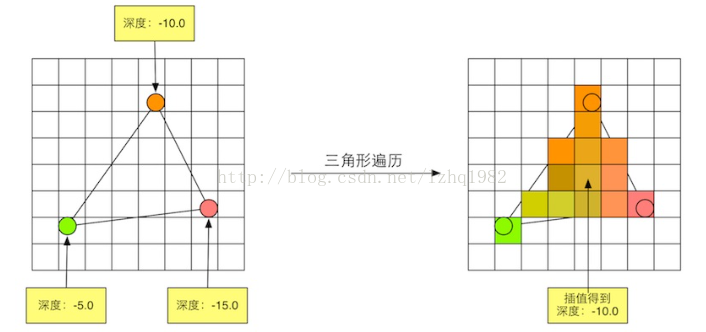
\includegraphics[width=.9\linewidth]{./pic/triangleTraverse.png}
\end{itemize}
\item 片元着色器
\label{sec-1-2-2-7}
\begin{itemize}
\item 片元着色器:又是我们重点关心的。这个阶段是可编程的(废话),上面的阶段给我们准备好了每个片元的所有数据,这个阶段就需要发挥你的能力用这些数据输出片元的颜色了,这里注意的是和前面的顶点着色器处理的单个顶点一样,这里我们处理的是单个片元,不要去想着访问其他片元。这个阶段可以做很多重要的渲染技术,比如纹理采样,用前面插值出来的纹理坐标采样出该片元对应的纹理颜色。
\end{itemize}
\item 逐片元操作
\label{sec-1-2-2-8}
\begin{itemize}
\item 逐片元操作:这个阶段的目的就是进行合并,是高度可配置的。有两个任务,一是经过一系列测试(模板测试、深度测试)决定每个片元的可见性,一是通过测试后留下的片元要和已存在颜色缓存区的颜色进行合并,开启混合的就混合,没开启的就直接覆盖。
\item 经过上面的所有计算后就该显示在屏幕上了,GPU采取多重缓冲的机制,渲染会发生在后置缓冲中,渲染结束后GPU可以交换到前置缓冲来显示。

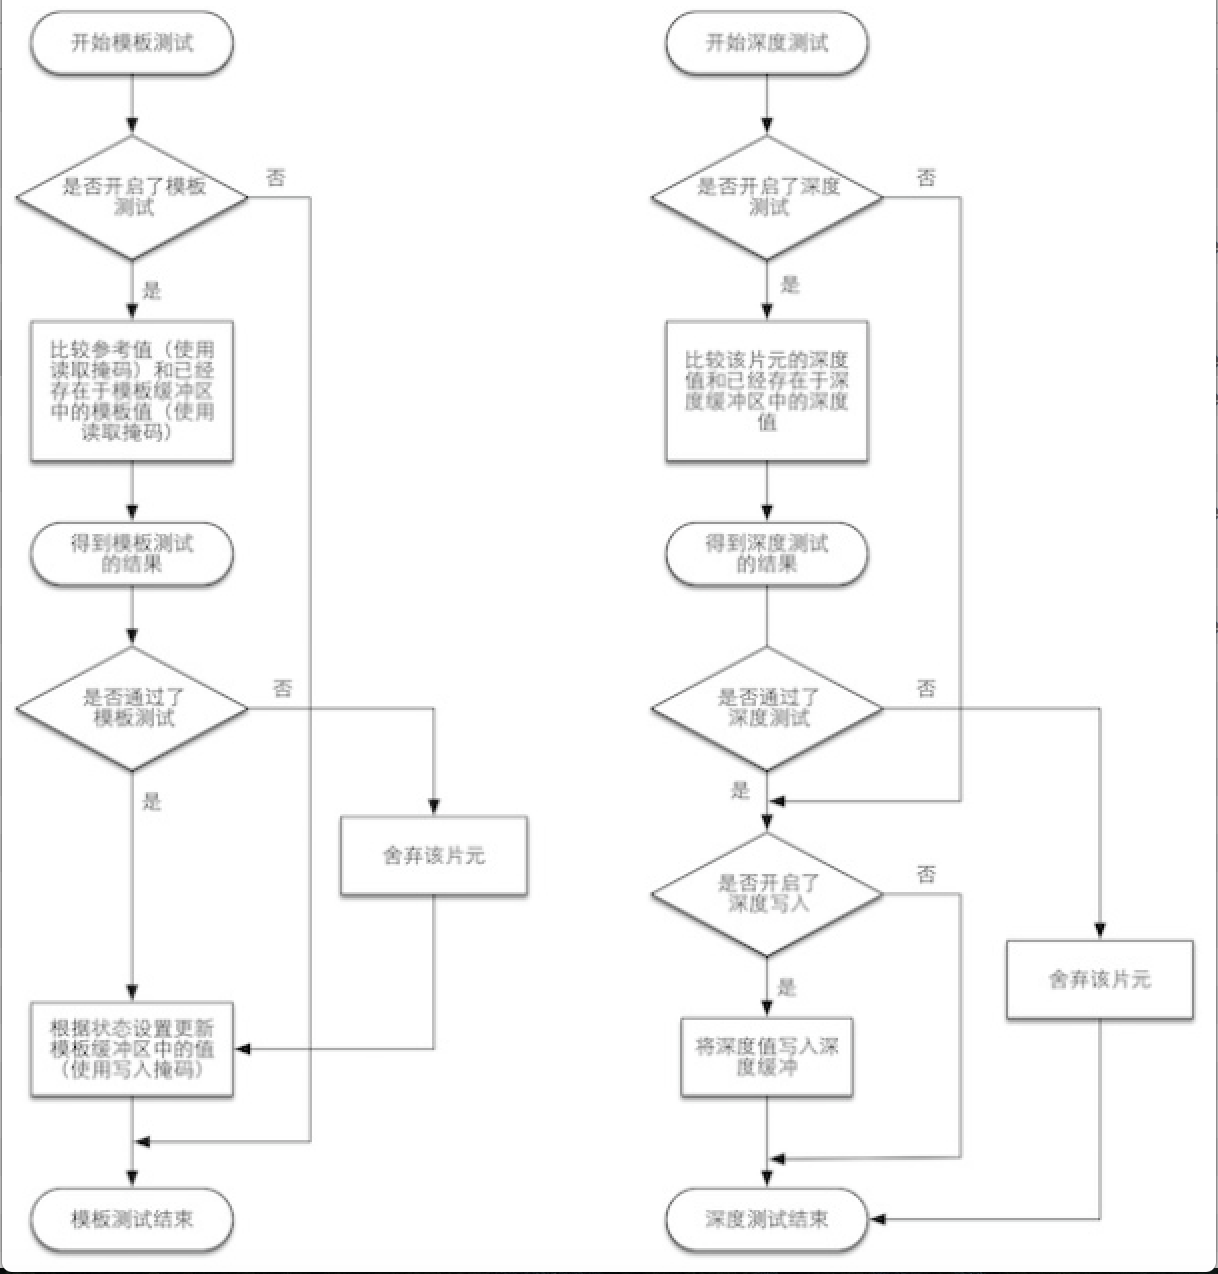
\includegraphics[width=.9\linewidth]{./pic/fragment.png}

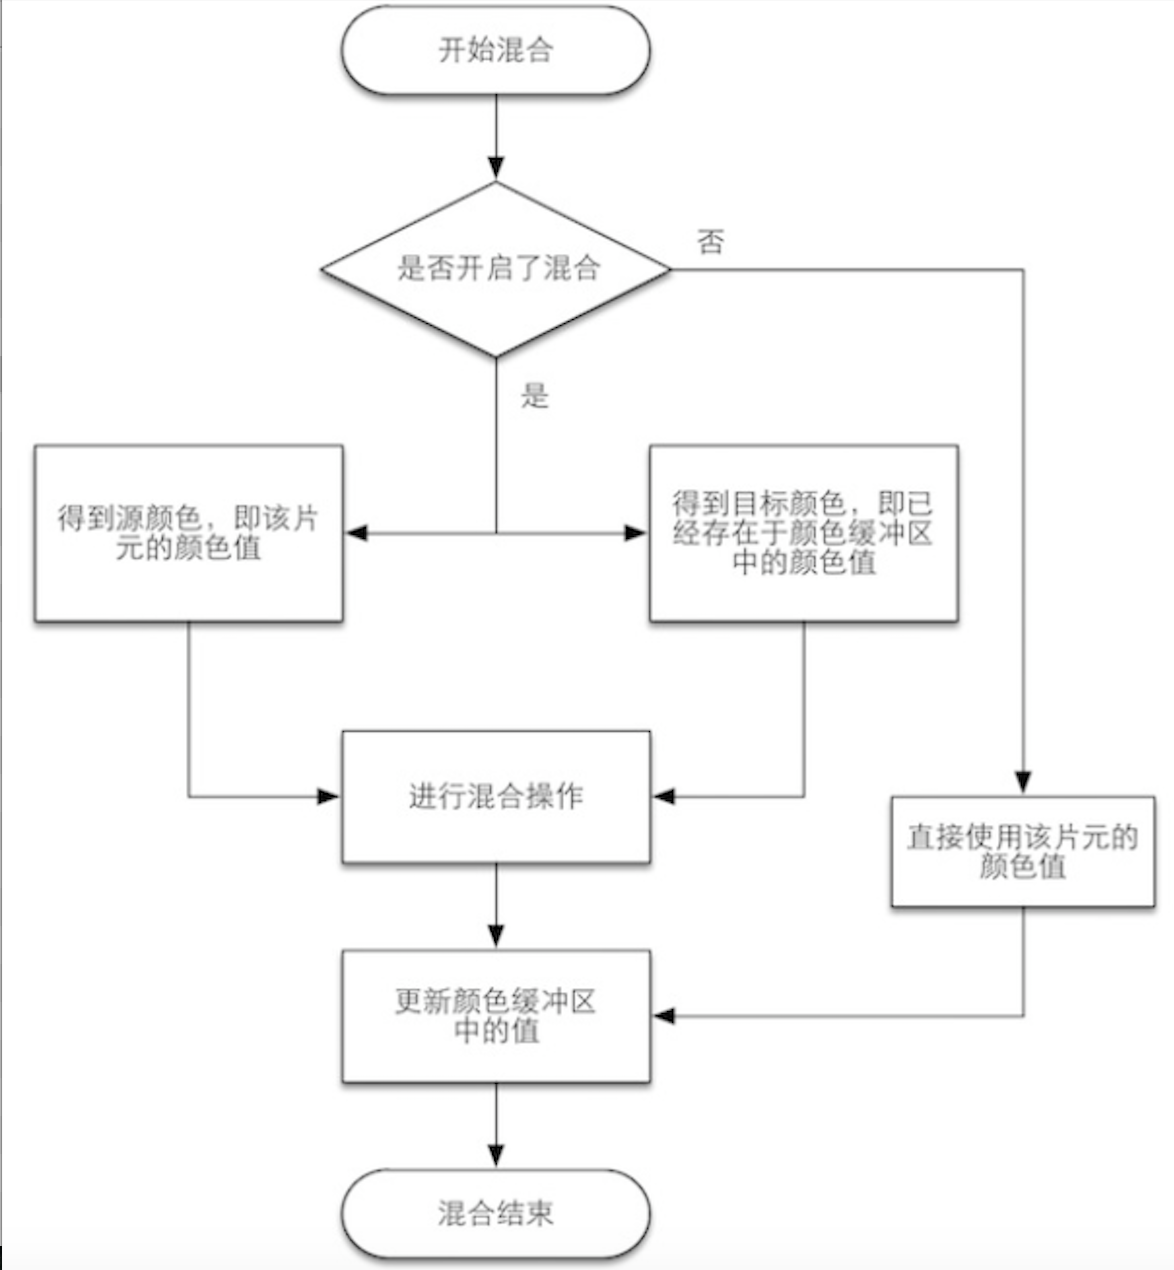
\includegraphics[width=.9\linewidth]{./pic/fragment2.png}
\end{itemize}
\end{enumerate}

\section{Unity Shader-渲染队列,ZTest,ZWrite,Early-Z}
\label{sec-2}
\begin{itemize}
\item \url{https://blog.csdn.net/puppet_master/article/details/53900568}
\end{itemize}
\subsection{简介}
\label{sec-2-1}
\begin{itemize}
\item 在渲染阶段,引擎所做的工作是把所有场景中的对象按照一定的策略(顺序)进行渲染。最早的是画家算法,顾名思义,就是像画家画画一样,先画后面的物体,如果前面还有物体,那么就用前面的物体把物体覆盖掉,不过这种方式由于排序是针对物体来排序的,而物体之间也可能有重叠,所以效果并不好。所以目前更加常用的方式是z-buffer算法,类似颜色缓冲区缓冲颜色,z-buffer中存储的是当前的深度信息,对于每个像素存储一个深度值,这样,我们屏幕上显示的每个像素点都会进行深度排序,就可以保证绘制的遮挡关系是正确的。而控制z-buffer就是通过ZTest,和ZWrite来进行。但是有时候需要更加精准的控制不同类型的对象的渲染顺序,所以就有了渲染队列。今天就来学习一下渲染队列,ZTest,ZWrite的基本使用以及分析一下Unity为了Early-Z所做的一些优化。
\end{itemize}
\subsection{Unity中的几种渲染队列}
\label{sec-2-2}
\begin{itemize}
\item 首先看一下Unity中的几种内置的渲染队列,按照渲染顺序,从先到后进行排序, \textbf{队列数越小的,越先渲染,队列数越大的,越后渲染。}
\end{itemize}
\begin{center}
\begin{tabular}{lrl}
\hline
Background & 1000 & 最早被渲染的物体的队列。\\
Geometry & 2000 & 不透明物体的渲染队列。大多数物体都应该使用该队列进行渲染,也是Unity Shader中默\\
 &  & 认的渲染队列。\\
AlphaTest & 2450 & 有透明通道,需要进行Alpha Test的物体的队列,比在Geomerty中更有效。\\
Transparent & 3000 & 半透物体的渲染队列。一般是不写深度的物体,Alpha Blend等的在该队列渲染。\\
Overlay & 4000 & 最后被渲染的物体的队列,一般是覆盖效果,比如镜头光晕,屏幕贴片之类的。\\
\hline
\end{tabular}
\end{center}
\begin{itemize}
\item Unity中设置渲染队列也很简单,我们不需要手动创建,也不需要写任何脚本,只需要在shader中增加一个Tag就可以了,当然,如果不加,那么就是默认的渲染队列Geometry。比如我们需要我们的物体在Transparent这个渲染队列中进行渲染的话,就可以这样写:
\begin{minted}[linenos=true]{csharp}
Tags { "Queue" = "Transparent"}
\end{minted}
\item 我们可以直接在shader的Inspector面板上看到shader的渲染队列:

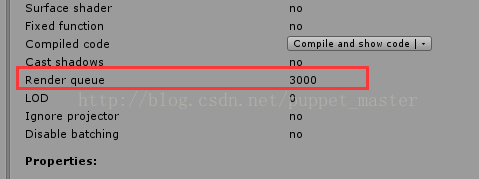
\includegraphics[width=.9\linewidth]{./pic/renderQueue.png}
\item 另外,我们在写shader的时候还经常有个Tag叫RenderType,不过这个没有Render Queue那么常用,这里顺便记录一下:
\begin{itemize}
\item \textbf{Opaque} : 用于大多数着色器(法线着色器、自发光着色器、反射着色器以及地形的着色器)。
\item \textbf{Transparent} : 用于半透明着色器(透明着色器、粒子着色器、字体着色器、地形额外通道的着色器)。
\item \textbf{TransparentCutout} : 蒙皮透明着色器(Transparent Cutout,两个通道的植被着色器)。
\item \textbf{Background} : 天空盒着色器。
\item \textbf{Overlay} : GUITexture,镜头光晕,屏幕闪光等效果使用的着色器。
\item \textbf{TreeOpaque} : 地形引擎中的树皮。
\item \textbf{TreeTransparentCutout} : 地形引擎中的树叶。
\item \textbf{TreeBillboard} : 地形引擎中的广告牌树。
\item \textbf{Grass} : 地形引擎中的草。
\item \textbf{GrassBillboard} : 地形引擎何中的广告牌草。
\end{itemize}
\end{itemize}
\subsection{相同渲染队列中不透明物体的渲染顺序}
\label{sec-2-3}
\begin{itemize}
\item 拿出Unity,创建三个立方体,都使用默认的bump diffuse shader(渲染队列相同),分别给三个不同的材质(相同材质的小顶点数的物体引擎会动态合批),用Unity5带的Frame Debug工具查看一下Draw Call。(Unity5真是好用得多了,如果用4的话,还得用NSight之类的抓帧)

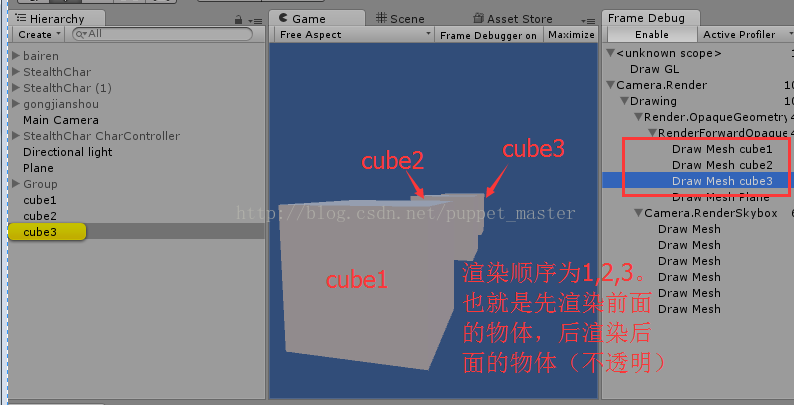
\includegraphics[width=.9\linewidth]{./pic/renderQueue1.png}
\item 可以看出,Unity中对于不透明的物体,是采用了从前到后的渲染顺序进行渲染的,这样,不透明物体在进行完vertex阶段,进行Z Test,然后就可以得到该物体最终是否在屏幕上可见了,如果前面渲染完的物体已经写好了深度,深度测试失败,那么后面渲染的物体就直接不会再去进行fragment阶段。(不过这里需要把三个物体之间的距离稍微拉开一些,本人在测试时发现,如果距离特别近,就会出现渲染次序比较乱的情况,因为我们不知道Unity内部具体排序时是按照什么标准来判定的哪个物体离摄像机更近,这里我也就不妄加猜测了)
\end{itemize}
\subsection{相同渲染队列中半透明物体的渲染顺序}
\label{sec-2-4}
\begin{itemize}
\item 透明物体的渲染一直是图形学方面比较蛋疼的地方,对于透明物体的渲染,就不能像渲染不透明物体那样多快好省了,因为透明物体不会写深度,也就是说透明物体之间的穿插关系是没有办法判断的,所以半透明的物体在渲染的时候一般都是采用从后向前的方法进行渲染,由于透明物体多了,透明物体不写深度,那么透明物体之间就没有所谓的可以通过深度测试来剔除的优化,每个透明物体都会走像素阶段的渲染,会造成大量的Over Draw。这也就是粒子特效特别耗费性能的原因。
\item 我们实验一下Unity中渲染半透明物体的顺序,还是上面的三个立方体,我们把材质的shader统一换成粒子最常用的Particle/Additive类型的shader,再用Frame Debug工具查看一下渲染的顺序:

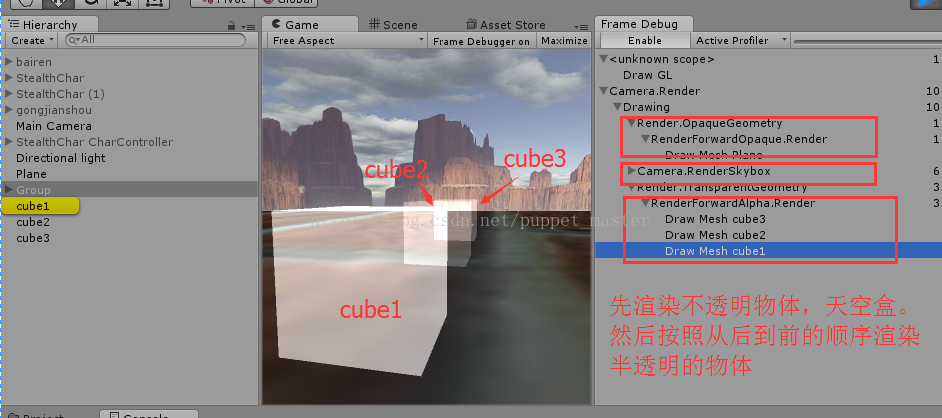
\includegraphics[width=.9\linewidth]{./pic/renderQueue2.png}
\end{itemize}
\subsection{自定义渲染队列}
\label{sec-2-5}
\begin{itemize}
\item Unity支持我们自定义渲染队列,比如我们需要保证某种类型的对象需要在其他类型的对象渲染之后再渲染,就可以通过自定义渲染队列进行渲染。而且超级方便,我们只需要在写shader的时候修改一下渲染队列中的Tag即可。比如我们希望我们的物体要在所有默认的不透明物体渲染完之后渲染,那么我们就可以使用Tag\{“Queue” = “Geometry+1”\}就可以让使用了这个shader的物体在这个队列中进行渲染。
\item 还是上面的三个立方体,这次我们分别给三个不同的shader,并且渲染队列不同,通过上面的实验我们知道,默认情况下,不透明物体都是在Geometry这个队列中进行渲染的,那么不透明的三个物体就会按照cube1,cube2,cube3进行渲染。这次我们希望将渲染的顺序反过来,那么我们就可以让cube1的渲染队列最大,cube3的渲染队列最小。贴出其中一个的shader:
\begin{minted}[linenos=true]{csharp}
Shader "Custom/RenderQueue1" {
 	SubShader {
		Tags {
            "RenderType"="Opaque" "Queue" = "Geometry+1"}
        Pass {
			CGPROGRAM
#pragma vertex vert
#pragma fragment frag
#include "UnityCG.cginc"
            struct v2f {
				float4 pos : SV_POSITION;
            };
            v2f vert(appdata_base v) {
				v2f o;
                o.pos = mul(UNITY_MATRIX_MVP, v.vertex);
                return o;
            }
            fixed4 frag(v2f i) : SV_Target {
				return fixed4(0,0,1,1);
            }
            ENDCG
        }
    }
    //FallBack "Diffuse"}
}
\end{minted}
\item 其他的两个shader类似,只是渲染队列和输出颜色不同。

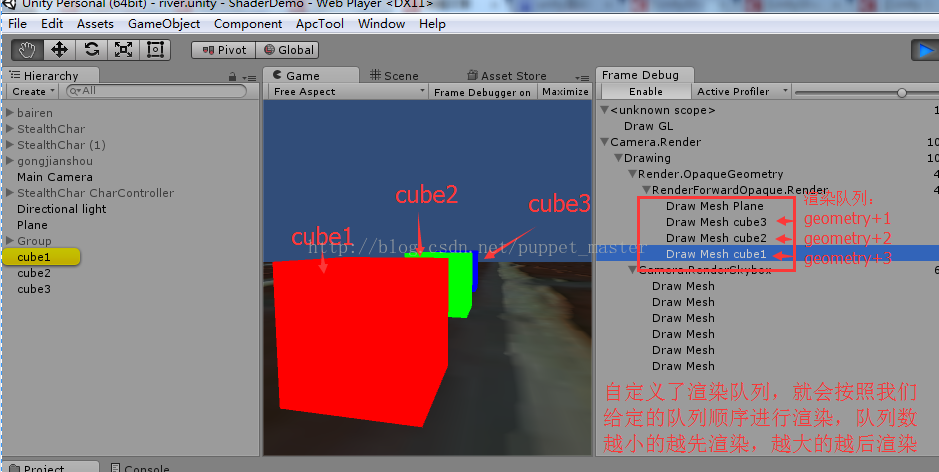
\includegraphics[width=.9\linewidth]{./pic/renderQueue3.png}
\item 通过渲染队列,我们就可以自由地控制使用该shader的物体在什么时机渲染。比如某个不透明物体的像素阶段操作较费,我们就可以控制它的渲染队列,让其渲染更靠后,这样可以通过其他不透明物体写入的深度剔除该物体所占的一些像素。
\item PS:这里貌似发现了个问题,我们在修改shader的时候一般不需要什么其他操作就可以直接看到修改后的变化,但是本人改完渲染队列后,有时候会出现从shader的文件上能看到渲染队列的变化,但是从渲染结果以及Frame Debug工具中并没有看到渲染结果的变化,重启Unity也没有起到作用,直到我把shader重新赋给材质之后,变化才起了效果\ldots{}(猜测是个bug,因为看到网上还有和我一样的倒霉蛋被这个坑了,本人的版本是5.3.2,害我差点怀疑昨天是不是喝了,刚实验完的结果就完全不对了\ldots{})
\end{itemize}
\subsection{ZTest(深度测试)和ZWrite(深度写入) }
\label{sec-2-6}
\begin{itemize}
\item 上一个例子中,虽然渲染的顺序反了过来,但是物体之间的遮挡关系仍然是正确的,这就是z-buffer的功劳,不论我们的渲染顺序怎样,遮挡关系仍然能够保持正确。而我们对z-buffer的调用就是通过ZTest和ZWrite来实现的。
\end{itemize}
\subsubsection{ZTest}
\label{sec-2-6-1}
\begin{itemize}
\item ZTest即深度测试,所谓测试,就是针对当前对象在屏幕上(更准确的说是frame buffer)对应的像素点,将对象自身的深度值与当前该像素点缓存的深度值进行比较,如果通过了,本对象在该像素点才会将颜色写入颜色缓冲区,否则否则不会写入颜色缓冲。ZTest提供的状态较多。
\begin{itemize}
\item \textbf{ZTest Less} (深度小于当前缓存则通过)
\item \textbf{ZTest Greater} (深度大于当前缓存则通过)
\item \textbf{ZTest LEqual} (深度小于等于当前缓存则通过)
\item \textbf{ZTest GEqual} (深度大于等于当前缓存则通过)
\item \textbf{ZTest Equal} (深度等于当前缓存则通过)
\item \textbf{ZTest NotEqual} (深度不等于当前缓存则通过)
\item \textbf{ZTest Always} (不论如何都通过)
\item 注意,*ZTest Off* 等同于 \textbf{ZTest Always} ,关闭深度测试等于完全通过。
\end{itemize}
\end{itemize}
\subsubsection{ZWrite}
\label{sec-2-6-2}
\begin{itemize}
\item ZWrite比较简单,只有两种状态, \textbf{ZWrite On} (开启深度写入)和 \textbf{ZWrite Off} (关闭深度写入)。当我们开启深度写入的时候,物体被渲染时针对物体在屏幕(更准确地说是frame buffer)上每个像素的深度都写入到深度缓冲区;反之,如果是ZWrite Off,那么物体的深度就不会写入深度缓冲区。但是,物体是否会写入深度,除了ZWrite这个状态之外,更重要的是需要深度测试通过,也就是ZTest通过,如果ZTest都没通过,那么也就不会写入深度了。就好比默认的渲染状态是ZWrite
\item On和ZTest LEqual,如果当前深度测试失败,说明这个像素对应的位置,已经有一个更靠前的东西占坑了,即使写入了,也没有原来的更靠前,那么也就没有必要再去写入深度了。所以上面的ZTest分为通过和不通过两种情况,ZWrite分为开启和关闭两种情况的话,一共就是四种情况:
\begin{itemize}
\item 1.深度测试通过,深度写入开启:写入深度缓冲区,写入颜色缓冲区;
\item 2.深度测试通过,深度写入关闭:不写深度缓冲区,写入颜色缓冲区;
\item 3.深度测试失败,深度写入开启:不写深度缓冲区,不写颜色缓冲区;
\item 4.深度测试失败,深度写入关闭:不写深度缓冲区,不写颜色缓冲区;
\end{itemize}
\item Unity中默认的状态(写shader时什么都不写的状态)是ZTest LEqual和ZWrite On,也就是说默认是开启深度写入,并且深度小于等于当前缓存中的深度就通过深度测试,深度缓存中原始为无限大,也就是说离摄像机越近的物体会更新深度缓存并且遮挡住后面的物体。如下图所示,前面的正方体会遮挡住后面的物体:

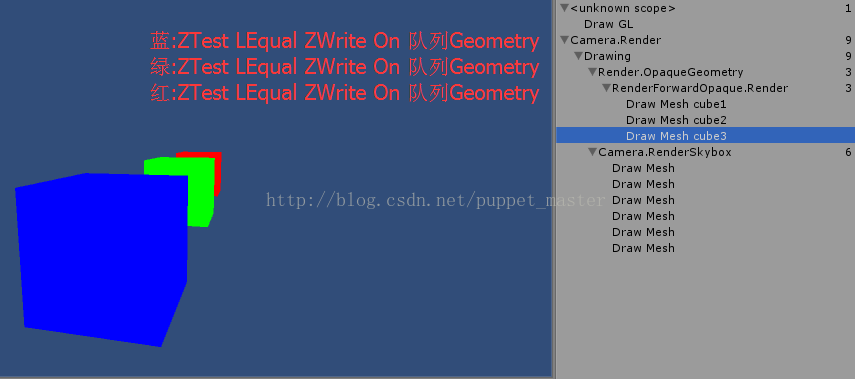
\includegraphics[width=.9\linewidth]{./pic/zwrite1.png}
\item 写几个简单的小例子来看一下ZTest,ZWrite以及Render Queue这几个状态对渲染结果的控制。
\item 让绿色的对象不被前面的立方体遮挡,一种方式是关闭前面的蓝色立方体深度写入:

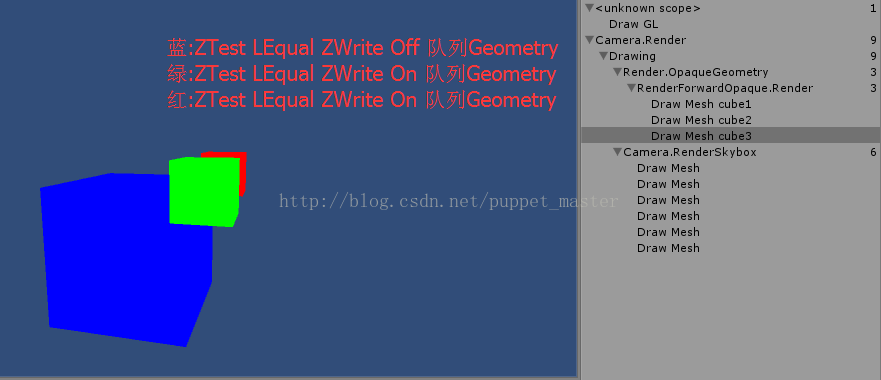
\includegraphics[width=.9\linewidth]{./pic/zwrite2.png}
\item 通过上面的实验结果,我们知道,按照从前到后的渲染顺序,首先渲染蓝色物体,蓝色物体深度测试通过,颜色写入缓存,但是关闭了深度写入,蓝色部分的深度缓存值仍然是默认的Max,后面渲染的绿色立方体,进行深度测试仍然会成功,写入颜色缓存,并且写入了深度,因此蓝色立方体没有起到遮挡的作用。
\item 另一种方式是让绿色强制通过深度测试:

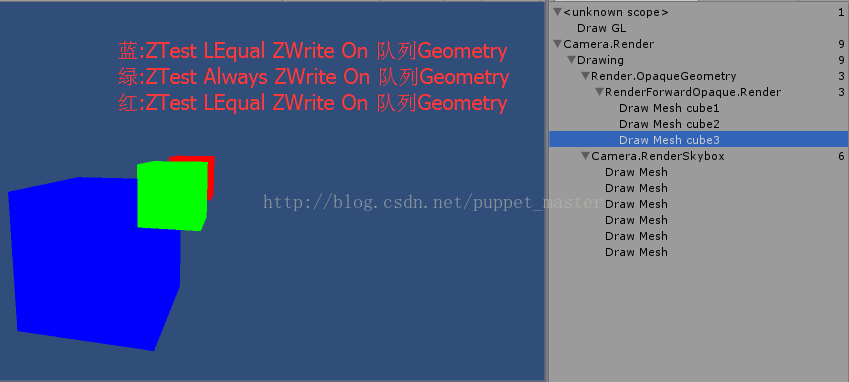
\includegraphics[width=.9\linewidth]{./pic/zwrite3.png}
\item 这个例子中其他立方体的shader使用默认的渲染方式,绿色的将ZTest设置为Always,也就是说不管怎样,深度测试都通过,将绿色立方体的颜色写入缓存,如果没有其他覆盖了,那么最终的输出就是绿色的了。
\item 那么如果红色的也开了ZTest Always会怎么样?

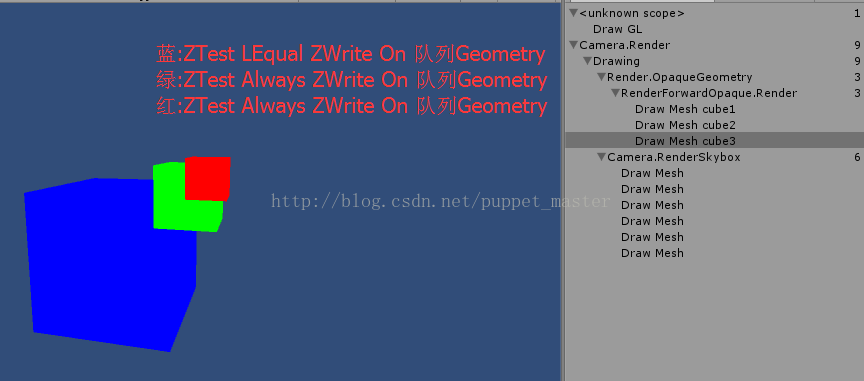
\includegraphics[width=.9\linewidth]{./pic/zwrite4.png}
\item 在红色立方体也用了ZTest Always后,红色遮挡了绿色的部分显示为了红色。如果我们换一下渲染队列,让绿色在红色之前渲染,结果就又不一样了:

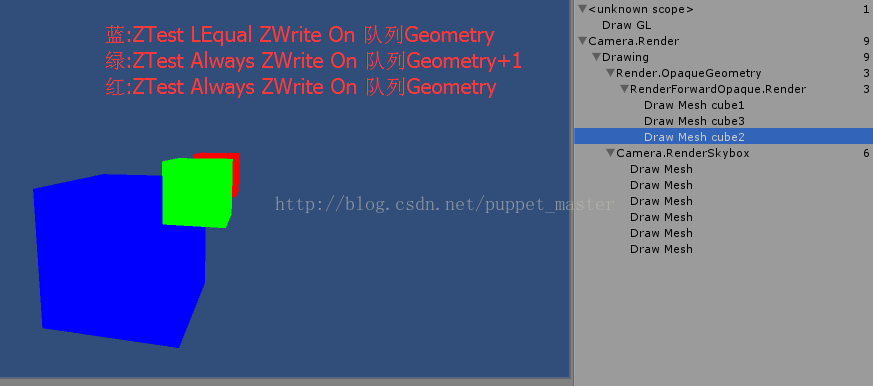
\includegraphics[width=.9\linewidth]{./pic/zwrite5.png}
\item 更换了渲染队列,让绿色的渲染队列+1,在默认队列Geometry之后渲染,最终重叠部分又变回了绿色。可见,当ZTest都通过时,上一个写入颜色缓存的会覆盖上一个,也就是说最终输出的是最后一个渲染的对象颜色。
\item 再看一下Greater相关的部分有什么作用,这次我们其他的都使用默认的渲染状态,绿色的立方体shader中ZTest设置为Greater:

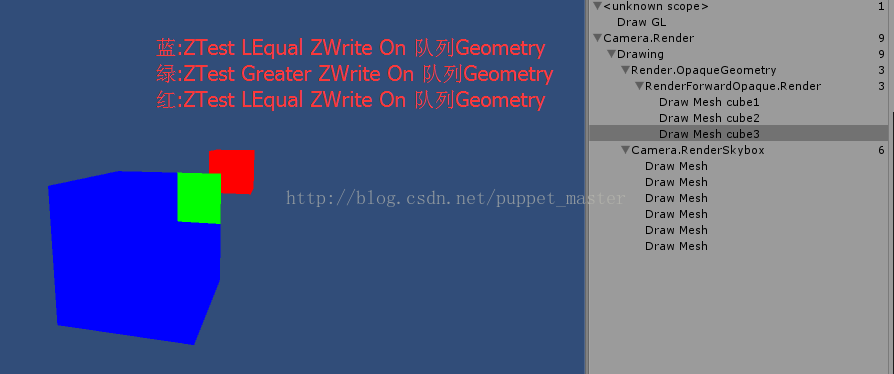
\includegraphics[width=.9\linewidth]{./pic/zwrite6.png}
\item 这个效果就比较好玩了,虽然我们发现在比较深度时,前面被蓝色立方体遮挡的部分,绿色的最终覆盖了蓝色,是想要的结果,不过其他部分哪里去了呢?简单分析一下,渲染顺序是从前到后,也就是说蓝色最先渲染,默认深度为Max,蓝色立方体的深度满足LEqual条件,就写入了深度缓存,然后绿色开始渲染,重叠的部分的深度缓存是蓝色立方体写入的,而绿色的深度值满足大于蓝色深度的条件,所以深度测试通过,重叠部分颜色更新为绿色;而与红色立方体重合的部分,红色立方体最后渲染,与前面的部分进行深度测试,小于前面的部分,深度测试失败,重叠部分不会更新为红色,所以重叠部分最终为绿色。而绿色立方体没有与其他部分重合的地方为什么消失了呢?其实是因为绿色立方体渲染时,除了蓝色立方体渲染的地方是有深度信息的,其他部分的深度信息都为Max,蓝色部分用Greater进行判断,肯定会失败,也就不会有颜色更新。
\item 有一个好玩的效果其实就可以考ZTest Greater来实现,就是游戏里面经常出现的,当玩家被其他场景对象遮挡时,遮挡的部分会呈现出X-光的效果;其实是在渲染玩家时,增加了一个Pass,默认的Pass正常渲染,而增加的一个Pass就使用Greater进行深度测试,这样,当玩家被其他部分遮挡时,遮挡的部分才会显示出来,用一个描边的效果渲染,其他部分仍然使用原来的Pass即可。
\end{itemize}
\subsection{Early-Z技术}
\label{sec-2-7}
\begin{itemize}
\item 传统的渲染管线中,ZTest其实是在Blending阶段,这时候进行深度测试,所有对象的像素着色器都会计算一遍,没有什么性能提升,仅仅是为了得出正确的遮挡结果,会造成大量的无用计算,因为每个像素点上肯定重叠了很多计算。因此现代GPU中运用了Early-Z的技术,在Vertex阶段和Fragment阶段之间(光栅化之后,fragment之前)进行一次深度测试,如果深度测试失败,就不必进行fragment阶段的计算了,因此在性能上会有很大的提升。但是最终的ZTest仍然需要进行,以保证最终的遮挡关系结果正确。前面的一次主要是Z-Cull为了裁剪以达到优化的目的,后一次主要是Z-Check,为了检查,如下图:

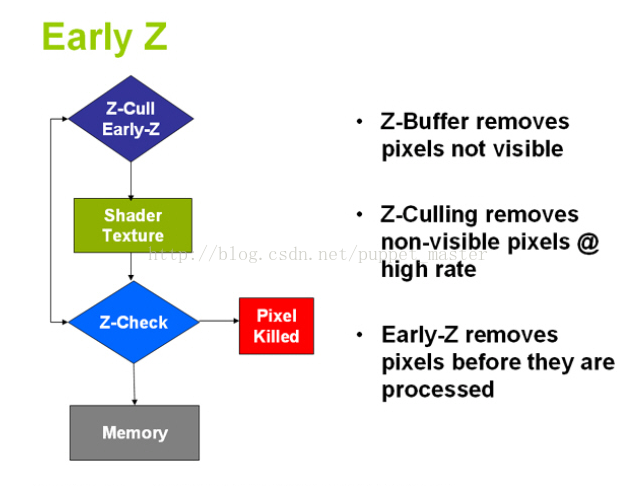
\includegraphics[width=.9\linewidth]{./pic/earlyz.png}
\item Early-Z的实现,主要是通过一个Z-pre-pass实现,简单来说,对于所有不透明的物体(透明的没有用,本身不会写深度),首先用一个超级简单的shader进行渲染,这个shader不写颜色缓冲区,只写深度缓冲区,第二个pass关闭深度写入,开启深度测试,用正常的shader进行渲染。其实这种技术,我们也可以借鉴,在渲染透明物体时,因为关闭了深度写入,有时候会有其他不透明的部分遮挡住透明的部分,而我们其实不希望他们被遮挡,仅仅希望被遮挡的物体半透,这时我们就可以用两个pass来渲染,第一个pass使用Color
\item Mask屏蔽颜色写入,仅写入深度,第二个pass正常渲染半透,关闭深度写入。
\item 关于Early-Z技术可以参考ATI的论文Applications of Explicit Early-Z Culling以及PPT,还有一篇Intel的文章。 
\begin{itemize}
\item \url{http://developer.amd.com/wordpress/media/2012/10/ShadingCourse2004_EarlyZ.pdf}
\item \url{http://amd-dev.wpengine.netdna-cdn.com/wordpress/media/2012/10/ShadingCourse_ATI.pdf}
\item \url{https://software.intel.com/en-us/articles/early-z-rejection-sample}
\end{itemize}
\end{itemize}
\subsection{Unity渲染顺序总结}
\label{sec-2-8}
\begin{itemize}
\item 如果我们先绘制后面的物体,再绘制前面的物体,就会造成over draw;而通过Early-Z技术,我们就可以先绘制较近的物体,再绘制较远的物体(仅限不透明物体),这样,通过先渲染前面的物体,让前面的物体先占坑,就可以让后面的物体深度测试失败,进而减少重复的fragment计算,达到优化的目的。Unity中默认应该就是按照最近距离的面进行绘制的,我们可以看一下Unity官方的文档中显示的:

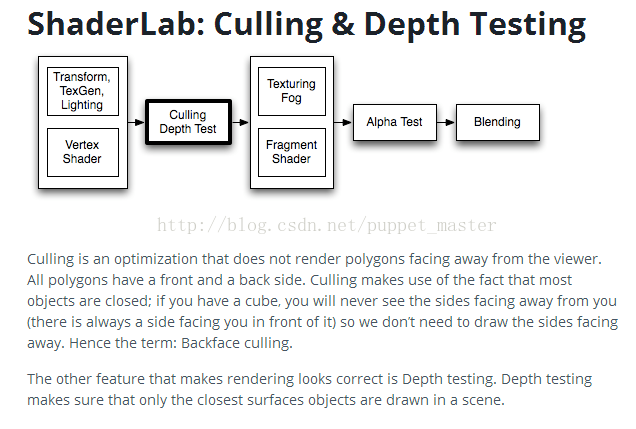
\includegraphics[width=.9\linewidth]{./pic/renderingOrder.png}
\item 从文档给出的流程来看,这个Depth-Test发生在Vertex阶段和Fragment阶段之间,也就是上面所说的Early-Z优化。
\item 简单总结一下Unity中的渲染顺序: \textbf{先渲染不透明物体,顺序是从前到后;再渲染透明物体,顺序是从后到前。}
\end{itemize}
\subsection{Alpha Test(Discard)在移动平台消耗较大的原因}
\label{sec-2-9}
\begin{itemize}
\item 从本人刚刚开始接触渲染,就开始听说移动平台Alpha Test比较费,当时比较纳闷,直接discard了为什么会费呢,应该更省才对啊?这个问题困扰了我好久,今天来刨根问底一下。还是跟我们上面讲到的Early-Z优化。正常情况下,比如我们渲染一个面片,不管是否是开启深度写入或者深度测试,这个面片的光栅化之后对应的像素的深度值都可以在Early-Z(Z-Cull)的阶段判断出来了;而如果开启了Alpha Test(Discard)的时候,discard这个操作是在fragment阶段进行的,也就是说这个面片光栅化之后对应的像素是否可见,是在fragment阶段之后才知道的,最终需要靠Z-Check进行判断这个像素点最终的颜色。其实想象一下也能够知道,如果我们开了Alpha Test并且还用Early-Z的话,一块本来应该被剃掉的地方,就仍然写进了深度缓存,这样就会造成其他部分被一个完全没东西的地方遮挡,最终的渲染效果肯定就不对了。所以,如果我们开启了Alpha Test,就不会进行Early-Z,Z Test推迟到fragment之后进行,那么这个物体对应的shader就会完全执行vertex shader和fragment shader,造成over draw。有一种方式是使用Alpha Blend代替Alpha Test,虽然也很费,但是至少Alpha Blend虽然不写深度,但是深度测试是可以提前进行的,因为不会在fragment阶段再决定是否可见,因为都是可见的,只是透明度比较低罢了。不过这样只是权宜之计,Alpha Blend并不能完全代替Alpha Test。
\item 关于Alpha Test对于Power VR架构的GPU性能的影响,简单引用一下官方的链接以及一篇讨论帖:

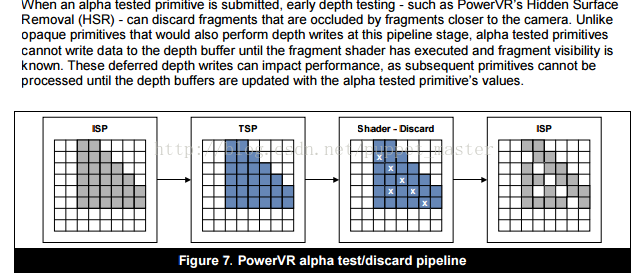
\includegraphics[width=.9\linewidth]{./pic/alphatest.png}
\end{itemize}
\subsection{最后再附上两篇参考文章}
\label{sec-2-10}
\begin{itemize}
\item \url{http://blog.csdn.net/candycat1992/article/details/41599167}
\item \url{http://blog.csdn.net/arundev/article/details/7895839}
\end{itemize}

\section{基础知识}
\label{sec-3}
\subsection{Unity影响渲染顺序因素的总结}
\label{sec-3-1}
\begin{itemize}
\item \url{https://blog.csdn.net/u011748727/article/details/68947207}
\end{itemize}
\subsubsection{Camera Depth}
\label{sec-3-1-1}
\begin{itemize}
\item 永远最高。Camera Depth小的一定先进渲染管线。
\end{itemize}
\subsubsection{2、当Sorting Layer和Order In Layer相同时}
\label{sec-3-1-2}
\begin{itemize}
\item RenderQueue小的先进渲染管线。
\end{itemize}
\subsubsection{当Sorting Layer和Order In Layer不相同时!}
\label{sec-3-1-3}
\begin{itemize}
\item 当两个材质使用了不同的RenderQueue,且这两个RenderQueue都在[0\textasciitilde{}2500]或[2501\textasciitilde{}5000]时,SortingLayer和OrderInLayer的排序生效。
\item 当两个材质使用了不同的RenderQueue,且这两个RenderQueue分别在[0\textasciitilde{}2500]和[2501\textasciitilde{}5000]时,则一定会按照RenderQueue绘制,无视SortingLayer、OrderInLayer的排序。
\end{itemize}

\subsection{specular镜面反射模型}
\label{sec-3-2}
\subsubsection{计算反射向量R的方法(unityCG函数库中reflect函数可用)}
\label{sec-3-2-1}

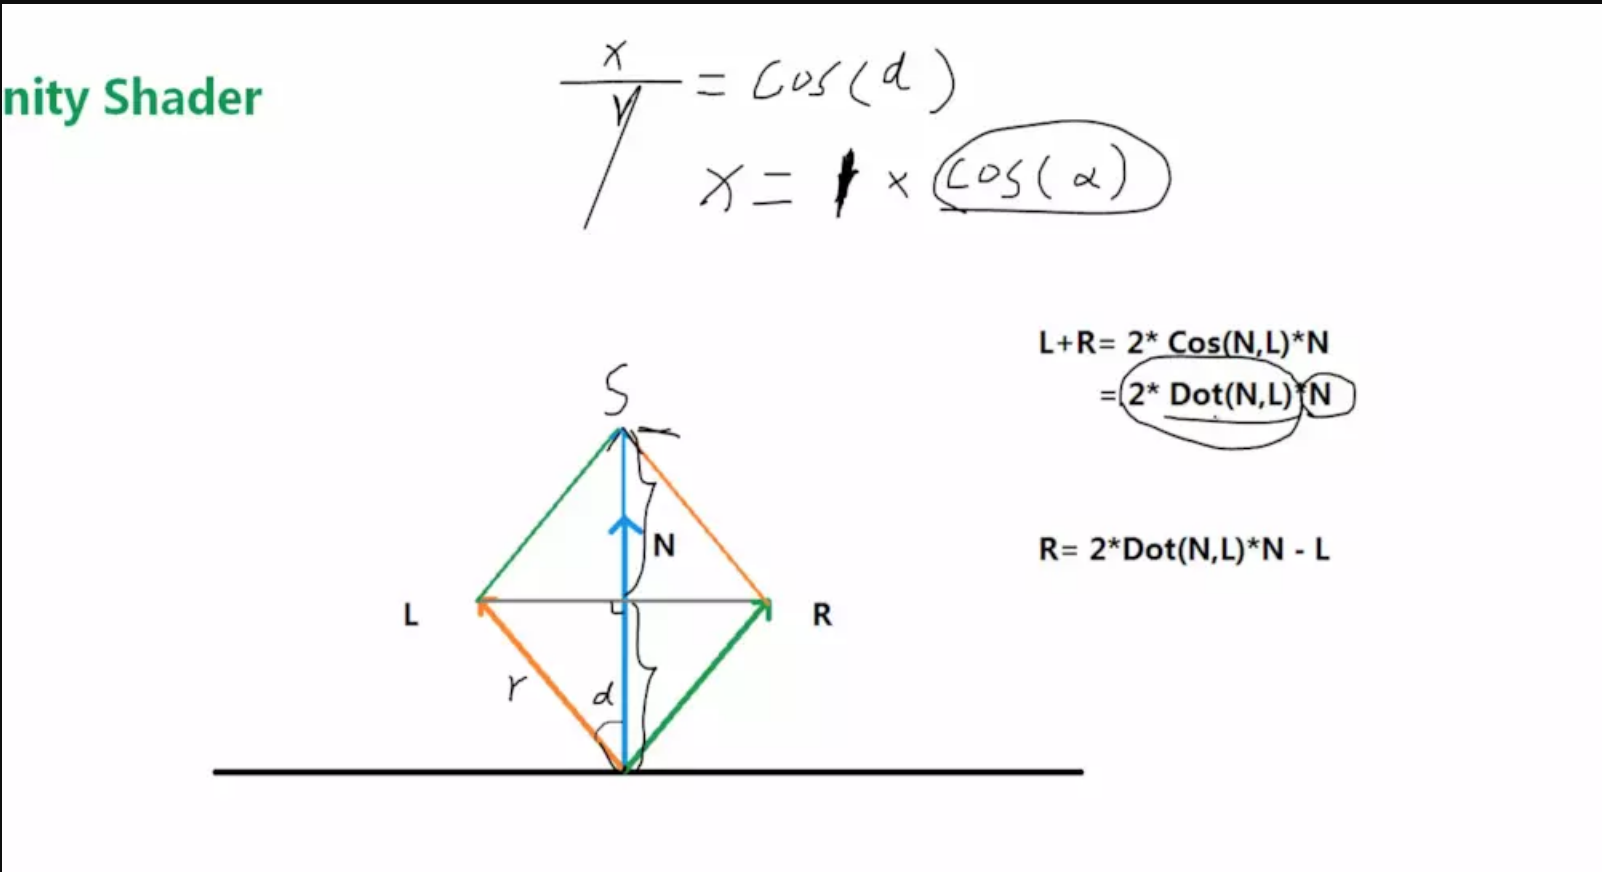
\includegraphics[width=.9\linewidth]{./pic/cosaNL2.png}
\subsubsection{phong模型,即环境光+漫反射+镜面反射模型}
\label{sec-3-2-2}
\begin{itemize}
\item 漫反射需要一次点积,镜面反射求反射向量时也要进行一次点积,但是下面的模型求镜面反射时不需要求反射向量,而是通过用入射向量(光)与平面指向摄像机的向量的和H来计算H与N的夹角,夹角越小,镜面反射越强
\end{itemize}
\subsubsection{blinnPhong模型,即在phong基础上进行一次点积优化的模型}
\label{sec-3-2-3}

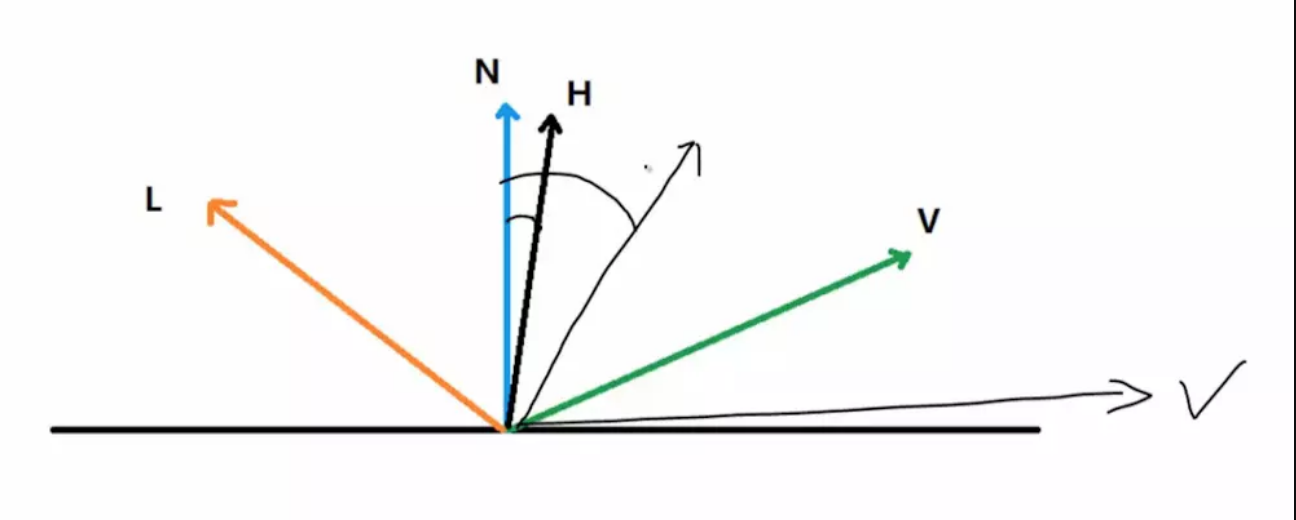
\includegraphics[width=.9\linewidth]{./pic/blinnphong.png}

\section{详解Unity3D Shader开发之渲染管线}
\label{sec-4}
\begin{itemize}
\item \url{https://blog.csdn.net/jxw167/article/details/54695181}
\item 我们需要知道面剔除操作是在渲染管线的哪个部分进行的,将渲染管线中的处理细化一下,效果如下所示:

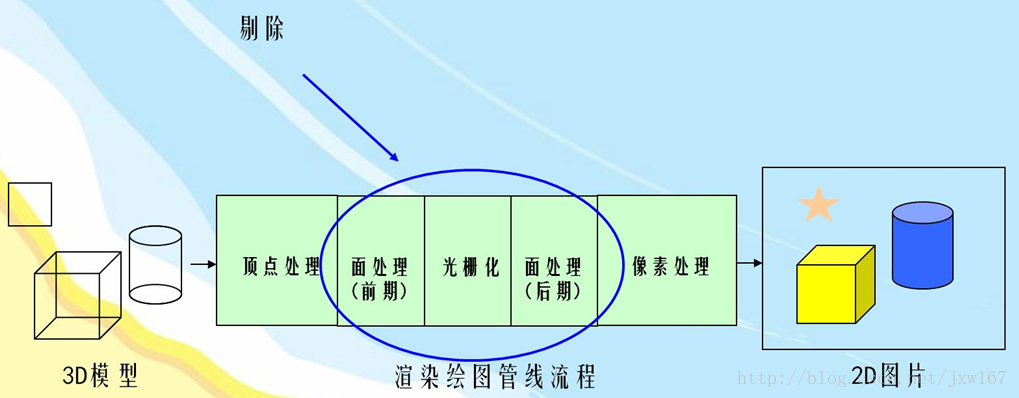
\includegraphics[width=.9\linewidth]{./pic/culling.png}
\item 渲染管线的流程是在GPU中进行的,展示效果如下所示:

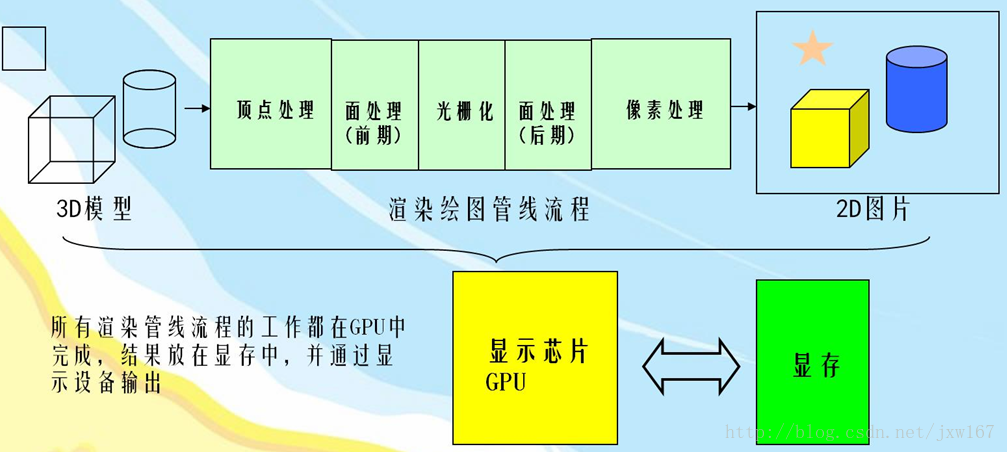
\includegraphics[width=.9\linewidth]{./pic/gpuculling.png}
\item 如果读者使用DirectX开发过Demo,对3D调用接口应该比较熟悉,下面结合着图片把在CPU中调用的接口对应到GPU使用的接口,展示效果如下所示:

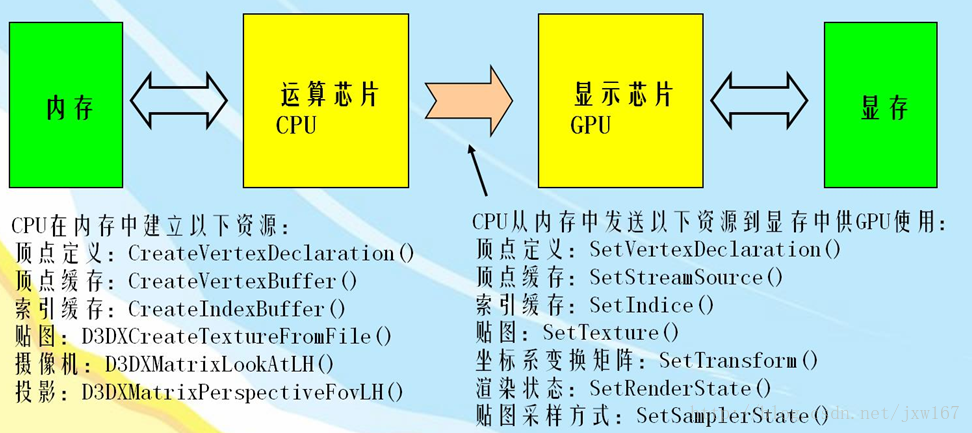
\includegraphics[width=.9\linewidth]{./pic/cullingfuncs.png}
\item 渲染管线主要分为四个步骤:顶点变换,图元装配,光栅化,像素处理,再结合着图片给读者介绍如下:

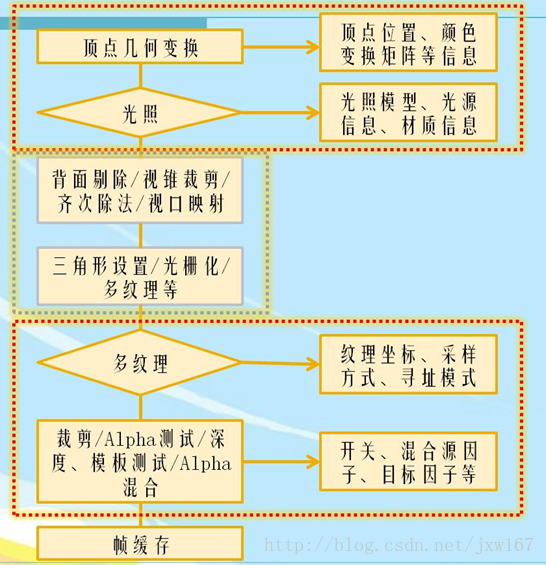
\includegraphics[width=.9\linewidth]{./pic/mvps.png}
\item Shader编程主要是分为两部分:一部分是顶点处理,一部分是像素处理。
\begin{itemize}
\item 顶点处理:顶点渲染的作用是对三维图元的顶点进行坐标变换和光照计算,生成可用于渲染到投影空间的顶点坐标、颜色和纹理坐标。顶点渲染就是定义了一系列针对顶点的渲染指令或渲染语句,当Direct3D处理图元顶点时,自动使用这些渲染指令或者渲染语句对每一个顶点逐一进行处理,完成顶点数据的处理工作。
\item 像素处理:对每个像素的颜色斤西瓜混合纹理采样,包括迭代颜色和纹理坐标、纹理采样以及将纹理采样与灯光和材质的颜色进行混合。比如:Alpha测试、深度测试、模版测试、计算每个像素的雾化值、Alpha混合等。
\end{itemize}
\end{itemize}
\section{Unity移动端性能优化}
\label{sec-5}
\begin{itemize}
\item \url{https://blog.csdn.net/poem_of_sunshine/article/details/71077171}
\end{itemize}
\subsection{渲染}
\label{sec-5-1}
\begin{itemize}
\item 利用reflect probe代替反射、折射,尽量不用RTT、GrabPass、RenderWithShader、CommandBuffer.Blit (BuiltinRenderTextureType.CurrentActive\ldots{})
\item 建立统一后处理框架(bloom、hdr、DOF等)代替多后处理,可以共用模糊函数,减少多次blit;另外要注意RTT的尺寸。
\item 空气折射、热浪扭曲等使用GrabPass不是所有硬件都支持,改为RTT或者后处理来优化。
\item 建立统一shader材质代替单一shader,充分利用shader$_{\text{feature、multi}}$$_{\text{compile,并将宏开关显示于界面。}}$
\item 图像混合代替多通道纹理,阴影投射、阴影接收、MetaPass、forwardadd 等pass不需要时要剔除。
\item 少用alpha test、discard、clip、Alpha Converage等,因为会影响Early-Z Culling、HSR的优化。
\item 避免Alpha Blend穿透问题(权重混合、深度剥离等透明排序方法代价太大了)。
\item 光照贴图代替动态阴影、尽量不用实时光;阴影贴图、环境贴图用16位代替32位;利用projector+rtt或者光圈代替实时阴影。
\item 将环境参数(风、雨、太阳)等shader全局参数统一管理。
\item 非主角可以用matcap代替pbr、无金属不一定要用pbr,仔细选择物理渲染所用的FDG(F:schlick、cook-torrance、lerp、要求不高用4次方,D:blinn-phong、beckmann、GGX、GGX Anisotropic,G:neumann、cook-torrance、Kelemen、SmithGGX;standard shader要注意选择BRDF1-BRDF3),渲染要求不高时不用GGX;可以用LH来优化GGX。
\item 用fixed、half代替float,建立shader统一类型(fixed效率是float的4倍,half是float的2倍),小心选择shader变量的修饰(uniform、static、全局),选择Mobile或Unlit目录下shader
\item 使用高低配渲染,内存足够时可以考虑开启mipmap
\item 使用surface shader注意关掉不用的功能,比如:noshadow、noambient、novertexlights、nolightmap、nodynlightmap、nodirlightmap、nofog、nometa、noforwardadd等
\item standard shader的变体太多(3万多),导致编译时间较长,内存占用也很惊人(接近1G),如果使用要关掉没用的shader$_{\text{feature}}$,比如:$_{\text{PARALLAXMAP、SHADOWS}}$$_{\text{SOFT、DIRLIGHTMAP}}$$_{\text{COMBINED}}$ DIRLIGHTMAP$_{\text{SEPARATE、}}$$_{\text{DETAIL}}$$_{\text{MULX2、}}$$_{\text{ALPHAPREMULTIPLY}}$$_{\text{ON;另外要去掉多余的pass}}$
\item shaderforge、Amplify Shader Editor生成的shader有多余代码要程序专门优化,Amplify Shader Editor功能更强大一些,而且开源,建议学习。
\item 不要用unity自带terrian,因为即使只用3张splat图,shader也是对应4个的,建议T4M或者转为mesh。
\item 模型和材质相同且数量巨大时用Instance来优化,比如草。
\item 利用查找纹理(LUT)来优化复杂的光照渲染,比如:皮肤、头发、喷漆等。
\item 尽量不要使用Procedural Sky,计算瑞丽散射和米氏散射效率比较低。
\item 尽量不要使用speedtree,改为模型加简单树叶动画,不过SpeedTreeWind.cginc里面的动画函数很丰富,TerrianEngine中的SmoothTriangleWave很好用。
\item 多用调试工具检查shader性能,常用工具有:FrameDebug、Nsight、RenderDoc 、AMD GPU ShaderAnalyzer / PVRShaderEditor、Adreno Profiler 、腾讯Cube、UWA等;另外可以内置GM界面,比如开关阴影,批量替换shader等方便真机调试。
\end{itemize}
\subsection{脚本}
\label{sec-5-2}
\begin{itemize}
\item 减少GetComponent、find等查找函数在Update等循环函数中的调用、go.CompareTag代替go.tag 、
\item 减少SendMessage等同步函数调用;减少字符串连接;for代替foreach,5.5以后版本foreach已经优化过了;少用linq;
\item 大资源改为异步加载
\item 合理处理协程调用
\item 将AI、网络等放在单独线程
\item 发布优化:关闭log、剔除代码
\item 伪随机
\item 脚本挂载类改为Manager等全局类实现
\item lua中尽量不实现update、fixedupdate等循环函数,lua和csharp互调用的效率比较低。
\end{itemize}
\subsection{内存管理}
\label{sec-5-3}
\begin{itemize}
\item 池子管理粒子、float UI等小资源,频繁地GC会造成卡顿
\item 必要时主动调用GC.Collect()
\item 按照不同资源、不同设备管理资源生命周期,Resources.Load和Assetbundle统一接口,利用引用计数来管理生命周期,并打印和观察生命周期。保证资源随场景而卸载,不常驻内存,确定哪些是预加载,哪些泄漏。
\item 内存泄漏(减少驻留内存):Container内资源不remove掉用Resources.UnloadUnusedAssets是卸载不掉的;对于这种情况,建议直接通过Profiler Memory中的Take Sample来对其进行检测,通过直接查看WebStream或SerializedFile中的AssetBundle名称,即可判断是否存在“泄露”情况;通过Android PSS/iOS Instrument反馈的App线程内存来查看;
\item 堆内存过大:避免一次性堆内存的过大分配,Mono的堆内存一旦分配,就不会返还给系统,这意味着Mono的堆内存是只升不降的。常见:高频调用new;log输出;
\item CPU占用高:NGui的重建网格导致UIPanel.LateUpdate(按照静止、移动、高频移动来切分);NGUI锚点自身的更新逻辑也会消耗不少CPU开销。即使是在控件静止不动的情况下,控件的锚点也会每帧更新(见UIWidget.OnUpdate函数),而且它的更新是递归式的,使CPU占用率更高。因此我们修改了NGUI的内部代码,使锚点只在必要时更新。一般只在控件初始化和屏幕大小发生变化时更新即可。不过这个优化的代价是控件的顶点位置发生变化的时候(比如控件在运动,或控件大小改变等),上层逻辑需要自己负责更新锚点。
\item 加载用协程; 控制同一个UIPanel中动态UI元素的数量,数量越多,所创建的Mesh越大,从而使得重构的开销显著增加。比如,战斗过程中的HUD血条可能会大量出现,此时,建议研发团队将运动血条分离成不同的UIPanel,每组UIPanel下5\textasciitilde{}10个动态UI为宜。这种做法,其本质是从概率上尽可能降低单帧中UIPanel的重建开销。
\item 资源冗余:AssetBundle打包打到多份中;动态修改资源导致的Instance拷贝多份(比如动态修改材质,Renderer.meterial,Animation.AddClip)。
\item 磁盘空间换内存:对于占用WebStream较大的AssetBundle文件(如UI Atlas相关的AssetBundle文件等),建议使用LoadFromCacheOrDownLoad或CreateFromFile来进行替换,即将解压后的AssetBundle数据存储于本地Cache中进行使用。这种做法非常适合于内存特别吃紧的项目,即通过本地的磁盘空间来换取内存空间
\end{itemize}
\subsection{美术}
\label{sec-5-4}
\begin{itemize}
\item 建立资源审查规范和审查工具:PBR材质贴图制作规范、场景制作资源控制规范、角色制作规范、特效制作规范;利用AssetPostprocessor建立审查工具。
\item 压缩纹理、优化精灵填充率、压缩动画、压缩声音、压缩UI(九宫格优于拉伸);严格控制模型面数、纹理数、角色骨骼数。
\item 粒子:录制动画代替粒子、减少粒子数量、粒子不要碰撞
\item 角色:启用Optimize Game Objects减少节点,使用(SimpleLOD、Cruncher)优化面数。
\item 模型:导入检查Read/Write only、Optimize Mesh、法线切线、color、禁用Mipmap
\item 压缩纹理问题:压缩可能导致色阶不足;无透明通道用ETC1,现在安卓不支持ETC2已不足5\%,建议放弃分离通道办法。
\item UI:尽可能将动态UI元素和静态UI元素分离到不同的UIPanel中(UI的重建以UIPanel为单位),从而尽可能将因为变动的UI元素引起的重构控制在较小的范围内; 尽可能让动态UI元素按照同步性进行划分,即运动频率不同的UI元素尽可能分离放在不同的UIPanel中; 尽可能让动态UI元素按照同步性进行划分,即运动频率不同的UI元素尽可能分离放在不同的UIPanel中;
\item ugui:可以充分利用canvas来切分不同元素。
\item 大贴图会导致卡顿,可以切分为多个加载。
\item iOS使用mp3压缩、Android使用Vorbis压缩
\end{itemize}
\subsection{批次}
\label{sec-5-5}
\begin{itemize}
\item 开启static batch
\item 开启dynamic batch:要求模型小于900顶点,用法线小于300,用切线小于180,缩放不一致、使用lightmap、多通道材质等会使dynamic batch无效。
\item 减少GameObject,场景模型数量对fps影响巨大。
\item 批次不是越少越好,过大的渲染数据会给总线传输带来压力。
\end{itemize}
\subsection{物理}
\label{sec-5-6}
\begin{itemize}
\item 不需要移动的物体设为Static
\item 不要用Mesh碰撞,角色不用碰撞体
\item 触发器逻辑优化
\item 寻路频率、AI逻辑频率 、Fixed Timestep、降帧到30
\item 出现卡顿的复杂计算,例如寻路、大量资源加载 可以用分帧或者协成异步来处理
\end{itemize}



\section{Unity性能优化(三)-图形渲染优化}
\label{sec-6}
\begin{itemize}
\item \url{https://blog.csdn.net/qq_21397217/article/details/80401708}
\end{itemize}
\subsection{渲染流程简介}
\label{sec-6-1}
\begin{itemize}
\item 在本文中,将会使用“对象”指代游戏中需要被渲染的对象,任何含有Renderer组件的GameObject都会被称为对象。
\item 通常使用 渲染管线 来描述渲染流程,其过程可以大致描述为:
\begin{itemize}
\item CPU决定哪些事物需要绘制以及它们如何被绘制。
\item CPU向GPU发送指令。
\item GPU根据CPU的指令对事物进行绘制。
\end{itemize}
\item 每渲染一帧画面,CPU都会进行如下工作:
\begin{itemize}
\item CPU检查场景中的每个对象来确定它是否需要进行渲染。只有满足指定条件的对象才会被渲染,例如:对象必须在相机的视锥体(Frustum)内并且没有被剔除(Culling)时才会被渲染。
\item CPU将每个需要渲染的对象的Mesh渲染数据编排到 Draw Call 指令中。某些情况下,一些共享配置的对象可能被合并到同一个Draw Call中,这个过程称为 批处理(Batching),参考Draw Call批处理手册。
\item CPU为每次Draw Call创建一个称为 Batch 的数据包。
\end{itemize}
\item 每次Draw Call,CPU要执行下列操作:
\begin{itemize}
\item CPU可能会向GPU发送 SetPass Call 指令来修改一些被统称为 Render State 的变量。每个SetPass Call都会告知GPU在下次渲染Mesh时要使用哪个配置。只有在下次需要渲染的Mesh的Render State与当前的Render State不同时,才会有SetPass Call。
\item CPU向GPU发送Draw Call指令。Draw Call指令告知GPU使用最近一次的SetPass Call的配置对指定的Mesh进行渲染。
\item 在某些情况下,一个Batch可能需要不止一个 Pass。Pass是一段Shader代码,新的Pass会改变Render State。CPU必须为Batch中的每个Pass发送新的SetPass Call并再次发送Draw Call。
\end{itemize}
\item 与此同时,GPU进行着如下的工作:
\begin{itemize}
\item GPU根据CPU的指令执行任务,执行顺序与指令发送顺序相同。
\item 如果当前的任务是一个SetPass Call,则GPU更新Render State。
\item 如果当前的任务是一个Draw Call,则GPU渲染Mesh。
\item 重复上述过程直到GPU将来自CPU的指令全部处理完。
\end{itemize}
\end{itemize}
\subsection{渲染问题的类型}
\label{sec-6-2}
\begin{itemize}
\item 引起渲染问题的基本原因有两个:
\begin{itemize}
\item 渲染管线(Rendering Pipeline)效率低,渲染管线中的一步或多步操作花费过多时间将导致数据流通不畅,这些低效问题被称为 瓶颈(Bottleneck)。
\item 在渲染管线中加入了太多数据,即使是在效率最高的渲染管线中,也有对一帧中处理的数据量的限制。
\end{itemize}
\item 如果游戏中因为CPU执行渲染任务耗时太久而导致帧渲染时间过长,我们称其为 CPU受限(CPU Bound)。
\item 如果游戏中因为GPU执行渲染任务耗时太久而导致帧渲染时间过长,我们称其为 GPU受限(GPU Bound)。
\end{itemize}
\subsection{处理CPU Bound}
\label{sec-6-3}
\begin{itemize}
\item 通常将帧渲染过程中的必须由CPU处理的任务分为三类:
\begin{itemize}
\item 决定什么必须被绘制
\item 为GPU准备指令
\item 向GPU发送指令
\end{itemize}
\item 这几个大类中包含很多独立的任务,这些任务可能被分散到多个线程中同时执行。在多个线程中执行渲染任务被称为 多线程渲染(Multithreaded Rendering)。
\item 在Unity的渲染过程中涉及了三中类型的线程:主线程(Main Thread)、渲染线程(Render Thread) 和 工作线程(Worker Thread)。主线程执行游戏中的大多数CPU任务,包括一些渲染任务;渲染线程专门用于向GPU发送指令;工作线程每次执行一个任务,例如剔除(Culling)或者蒙皮(Mesh Skining),CPU核数越多,可以创建的工作线程就越多。
\item 并不是所有的平台都支持多线程渲染,比如,目前的(Unity 5.4)WebGL平台就不支持多线程渲染。在不支持多线程渲染的平台上,所有的CPU任务都在同一个线程中处理。
\end{itemize}
\subsubsection{使用图形作业(Graphics Jobs)功能}
\label{sec-6-3-1}
\begin{itemize}
\item Player Settings 中的Graphics jobs选项可以让Unity将那些本该由主线程处理的渲染任务分配到工作线程中,有些时候也会把渲染线程的任务分配到工作线程。在可以使用该功能的平台上,它将带来显著的性能提升。该功能目前(Unity 2018.1.0)仍处于试验阶段,可能造成游戏崩溃。
\end{itemize}
\subsubsection{减少向GPU发送的数据量}
\label{sec-6-3-2}
\begin{itemize}
\item 向GPU发送指令的时间开销是引起CPU Bound的最常见原因。该过程在大多数平台上都会分配到渲染线程中执行,但在某些平台(比如PlayStation 4)上会分配到工作线程中执行。
\item 向GPU发送指令的过程中,开销最大的操作是SetPass Call。如果游戏在向GPU发送指令的过程中发生了CPU Bound,那么降低SetPass Call数量可能是最好的提升性能方式。通常,降低Batch数目、让更多的对象共享相同的Render State会降低SetPass Call数目,进而提高CPU性能。即使降低Batch数目没能够让SetPass Call数目降低,它也能提升性能,因为CPU处理单个Batch的能力比处理多个Batch的能力更强,即使这些Batch中包含的Mesh数据量是相同的。
\item 通常,有3种 降低Batch和SetPass Call数目的方法:
\begin{itemize}
\item 降低需要渲染的对象的数量,可以同时减少Batch和SetPass Call。
\item 降低每个对象需要被渲染的次数,可以减少SetPass Call。
\item 将对象合并到更少的批处理当中,可以减少Batch。
\end{itemize}
\end{itemize}
\subsubsection{降低需要渲染的对象的数量}
\label{sec-6-3-3}
\begin{itemize}
\item 减少Scene中可见的对象数量。
\item 缩短相机绘制距离。使用相机的 Far Clip Plane 属性控制相机的绘制距离,可以使用雾(Fog)掩饰远处缺失的对象。
\item 在代码中设置相机的 Layer Cull Distances 属性来更细致地控制相机在不同层(Layer)地绘制距离。
\item 使用相机地 遮挡剔除(Occlusion Culling) 选项关闭对被其他对象遮挡地对象地渲染。遮挡剔除并不适用于所有Scene,它会造成额外的CPU开销。这篇博客讲述了更多关于遮挡剔除地内容。
\end{itemize}
\subsubsection{降低每个对象需要被渲染的次数}
\label{sec-6-3-4}
\begin{itemize}
\item 实时光照、阴影和反射可以增强游戏地真实性,但使用这些特性会导致对象被渲染多次,很影响性能。这些特性所造成地具体影响取决于游戏所使用的 渲染通道(Rendering Path)。渲染通道是指绘制Scene时的运算的执行顺序,不同渲染通道间的主要区别是处理实时光照、阴影和反射的方式。通常来说,运行在高性能机器上并且使用了较多实时光照、阴影和反射的游戏适合使用 Deferred Rendering,而运行在低性能机器上并且没有使用这些特性的游戏适合使用 Forward Rendering。
\item 使用 烘培(Baking) 预先计算那些不会发生变化的对象的光照信息,减少实时光照的计算量。
\item 在 Quality Settings 中调整阴影属性,控制阴影质量。
\item 尽量少用 反射探针(Reflection Probe),它们会导致Batch数量大量增加。
\item Unity手册中对渲染通道进行了更多讲解。
\item 光照与渲染介绍中对Unity的光照进行了详细的讲解。
\end{itemize}
\subsubsection{将对象数据合并到更少的Batch当中}
\label{sec-6-3-5}
\begin{itemize}
\item 关于批处理优化的详细介绍,参考开头提到的那篇文章:【Unity技巧】Unity中的优化技术 。
\item 一个批处理中可以包含多个对象的数据,前提是这些对象满足下列条件:
\begin{itemize}
\item 共用同一个材质(Material)的同一个实例。
\item 拥有相同的材质设置(例如:纹理、Shader和Shader参数)。
\end{itemize}
\item 批处理可以提升性能,但是要小心使用,以免批处理过程的开销比其节省的开销还要高。
\item 对于满足批处理条件的对象,有几种不同的优化技术:
\begin{itemize}
\item \textbf{静态批处理(Static Batching)} :用于处理临近的静态对象(被标记为Batching Static),会占用更多的内存。
\item \textbf{动态批处理(Dynamic Batching)} :用于处理非静态对象,它的限制比较多,而且会占用更多的CPU时间。
\item \textbf{UI批处理} :对UI的批处理比较复杂,它受UI布局的影响,请参考Unity UI优化指导。
\item \textbf{GPU实例(GPU Instancing)} :用于处理集中出现的大量的独立对象,例如粒子。GPU实例的限制比较多,而且需要硬件支持,请参考GPU实例手册。
\item \textbf{纹理图集(Texture Atlasing)} :将多个纹理贴图合并到一张大的纹理贴图中。
\item \textbf{手动合并Mesh} :通过Unity编辑器或者代码将共用相同材质和纹理的Mesh合并。手动合并Mesh会影响对象的剔除,请参考Mesh.CombineMeshes。
\end{itemize}
\item 在代码中要谨慎使用 Renderer。material ,他会将material对象复制一份并非返回新对象的引用。这会破坏对象的批处理条件,因为Renderer不再持有与其他对象共用的材质的实例。如果要在代码中获取批处理对象的材质,应该使用 Renderer.sharedMaterial,参考Draw Call批处理手册。
\end{itemize}
\subsubsection{剔除、排序和批处理优化}
\label{sec-6-3-6}
\begin{itemize}
\item 剔除、获取需要渲染的对象的数据、将数据排序到批处理中以及生成GPU指令都能导致CPU受限。这些任务可以在主线程或者独立的工作线程中执行,具体取决于游戏设置和目标硬件平台。
\begin{itemize}
\item 剔除操作本身的开销不算太高,但减少不必要的剔除仍可以提升性能。Scene中的每个激活(active)的相机和对象都会产生开销,应该禁用(disable)那些当前不适用的相机和Renderer。
\item 批处理可以极大的提升向GPU发送指令的速度,但有时他可能造成意想不到的开销。如果批处理造成了CPU受限,就应该限制游戏中手动/自动批处理的数量。
\end{itemize}
\end{itemize}
\subsubsection{蒙皮(Skinned Meshes)优化}
\label{sec-6-3-7}
\begin{itemize}
\item SkinnedMeshRenderer 组件用于处理骨骼动画,常用在角色动画上。与蒙皮相关的任务可以在主线程或者独立的工作线程中执行,具体取决于游戏设置和目标硬件平台。
\item 蒙皮渲染的开销比较高,下面一些 对蒙皮渲染进行优化的手段:
\begin{itemize}
\item 减少SkinnedMeshRenderer组件的数量。导入模型时,模型可能带有SkinnedMeshRenderer组件,如果游戏中该模型并不会使用骨骼动画,就应该将SkinnedMeshRenderer组件替换为MeshRenderer。在导入模型时,可以选择不导入动画,请参考模型导入设置。
\item 减少使用SkinnedMeshRenderer的对象的Mesh顶点数,参考蒙皮渲染器手册。
\item 使用GPU Skinning。在硬件平台支持并且GPU资源足够的条件下,可以在Player Setting中启用GPU Skinning,将蒙皮任务从CPU转移到GPU。
\end{itemize}
\item 更多优化内容请参考角色模型优化手册。
\end{itemize}
\subsubsection{减少主线程中与渲染无关的操作}
\label{sec-6-3-8}
\begin{itemize}
\item 很多与渲染无关的任务都主线程中执行,减少主线程中与渲染无关的任务的CPU时间消耗。
\end{itemize}
\subsection{处理GPU Bound}
\label{sec-6-4}
\subsubsection{优化填充率(Fill Rate)}
\label{sec-6-4-1}
\begin{itemize}
\item 填充率指GPU每秒能够渲染的屏幕像素数量,它是引起GPU的性能问题的最常见因素,尤其是在移动设备上。下面列出一些 与填充率相关的优化手段:
\begin{itemize}
\item 优化 \textbf{片元着色器(Fragment Shader)} 。片元着色器是用于控制GPU如何绘制单个像素的Shader代码段,绘制每个像素点都需要执行这段代码。复杂的片元着色器是引起填充率问题的常见原因。 
\begin{itemize}
\item 如果在使用Unity内置Shader,优先使用能够满足视觉效果要求的最简单高效的Shader。例如,Unity内置的几种适用于移动平台的Mobile Shader都经过高度优化,而且它们也可以于移动平台以外的其他平台,如果它们提供的视觉效果能够满足需求,就应该使用这些Shader。
\item 如果在使用Unity提供的Standard Shadar,Unity会根据当前的材质设置对Shader进行编译,只有当前使用了的属性才会被编译。这意味着,移除材质中的一些可以省略的属性(例如Secondary Maps(Detail Maps))能够提升性能。
\end{itemize}
\end{itemize}
\end{itemize}
如果在使用自行编写的Shader,应该尽可能对其进行优化,请参考Shader优化提示。
\begin{itemize}
\item 减少 \textbf{重绘(Overdraw)} 。重绘指对同一个像素点进行多次绘制,这种情况发生在对象被绘制在其他对象上层时,它会极大地增加填充率。最常见地引起过渡重绘地因素是透明材质、未经优化地粒子和重叠地UI元素,应该对这些内容进行优化或者减少使用量。请参考:渲染队列、子着色器标签和填充率、画布和输入。
\item 减少 \textbf{图像特效(Image Efficts)} 。图像特效是引起填充率问题的重要因素,尤其是在使用了多个图像特效时。在同一个相机上使用多个图像特效会产生多个Shader Pass,将多个图像特效的Shader代码合并到单个Pass中可以提升性能,参考后期处理。
\end{itemize}
\subsubsection{优化显存带宽(Memory Bandwidth)}
\label{sec-6-4-2}
\begin{itemize}
\item 显存带宽指GPU对其专用的内存的读写速率。如果游戏出现带宽受限,通常是因为使用了太大的纹理(Texture)。
\item 优化纹理的方法:
\begin{itemize}
\item 纹理压缩(Texture Compression)可以极大的减少内存和磁盘占用。
\item Mipmap 是用在远处的物体上的低分辨率版本纹理。如果游戏中需要显示离相机很远的物体,则可以使用Mipmap减少显存带宽占用。
\end{itemize}
\item 纹理优化的具体细节,请参考纹理手册。
\end{itemize}
\subsubsection{优化顶点处理(Vertex Processing)}
\label{sec-6-4-3}
\begin{itemize}
\item 顶点处理指GPU渲染Mesh中的每个顶点使所做的工作。顶点处理的开销与两个因素有关:需要进行渲染的顶点的数量和对每个顶点所要进行的操作。
\item 优化顶点处理方法:
\begin{itemize}
\item 降低Mesh复杂度。
\item 使用 \textbf{法线贴图(Normal Map)} ,请参考法线贴图手册。
\item 禁用不使用法线贴图的模型的 顶点切线,这可以减少每个顶点发送给GPU的数据量,请参考模型导入设置。
\item 使用 \textbf{LOD} ,让物体根据离相机的距离展示不同的细节,请参考LOD组手册。
\item 降低 \textbf{顶点着色器(Vertex Shadar)} 代码复杂度。顶点着色器是用于控制GPU如何绘制每个顶点的Shader代码段,优化方式请参考片元着色器优化方式的第1、3条。
\end{itemize}
\end{itemize}

\section{Unity技巧】Unity中的优化技术}
\label{sec-7}
\begin{itemize}
\item \url{https://blog.csdn.net/candycat1992/article/details/42127811}
\end{itemize}
% Emacs 25.3.1 (Org mode 8.2.7c)
\end{document}